\documentclass{amsart}
\usepackage{graphicx}
\graphicspath{{./}}
\usepackage{hyperref}
\usepackage{csvsimple}
\usepackage{longtable}
\usepackage{epigraph}
\title{How Much Faith Do I have in the Human Race?}
\author{Zulfikar Moinuddin Ahmed}
\date{\today}
\begin{document}
\maketitle


\section{I Have Complete Faith in The Human Race}

I have been on Earth for 48 years, and not even for a moment did I have any lack of faith in the Human Race.  Now this is not a matter of simple and stubborn conviction.  It is because I am only having a human life because I am an Archangel of Heaven having a human life.  Why would I choose a human life without having faith in the Human Race?

\section{The Scope of my Faith in the Human Race}

Human Race is a relatively young, relatively primitive Angelic Race.  It does not even know that it is a Single Race, and its peoples are divided and in conflict across the globe.  There is a goddam Demon in America plotting tribal dominance and slavery across the world.  The Human Race is not like one of the finely refined Angelic Races that have resolved these elementary problems several hundred thousand years ago.  It is a Primitive Mercantile Age.  Human Race is not even in contact with advanced Angelic Civilisations who are quite far away.  So what does it {\em mean} when I say I have faith in the Human Race?  

Well I am an Angel Soul, so I am quite aware of how slowly things develop in this sort of Angelic World.  It will be several thousand years before the coherence of Human Race is quite clear.  I could reduce the stress on Money on Earth with my Global Individual Debt project.  But that is not certain.

\section{Key Lesson}

Do not decide to have faith or not faith in any Race at all based on your personal interactions with a small sample.  Only a truly ignorant Angel would pretend that the entire Race can be assessed in this manner.  The Human Race has 7.8 billion and there are other means of assessing it accurately.  I have proven that the Human Race is an Angelic Race.  Now Angelic Races do not automatically gain perfection of Civilisation.  

\section{I Do Not Stubbornly Hold on to Unrealistic Optimistic View of Human Race}

I love human poetry.  Consider Yeats' "The Second Coming".

BY WILLIAM BUTLER YEATS

Turning and turning in the widening gyre   
The falcon cannot hear the falconer;
Things fall apart; the centre cannot hold;
Mere anarchy is loosed upon the world,
The blood-dimmed tide is loosed, and everywhere   
The ceremony of innocence is drowned;
The best lack all conviction, while the worst   
Are full of passionate intensity.

Surely some revelation is at hand;
Surely the Second Coming is at hand.   
The Second Coming! Hardly are those words out   
When a vast image out of Spiritus Mundi
Troubles my sight: somewhere in sands of the desert   
A shape with lion body and the head of a man,   
A gaze blank and pitiless as the sun,   
Is moving its slow thighs, while all about it   
Reel shadows of the indignant desert birds.   
The darkness drops again; but now I know   
That twenty centuries of stony sleep
Were vexed to nightmare by a rocking cradle,   
And what rough beast, its hour come round at last,   
Slouches towards Bethlehem to be born?


There is a pessimism in the poetry; this pessimism is not wrong in a sense.  You see a Demon with money and power and an Angel who could consider himself being mistreated by the world.  But that's only a mood, a viewpoint.  Angels cannot simply live in the rather self-absorbed melancholy.  We have greater duties.  I like the Human Race, and I am happy to advocate for Humans among Angels.

\section{Picture of Gaza in New York Times Front Page}

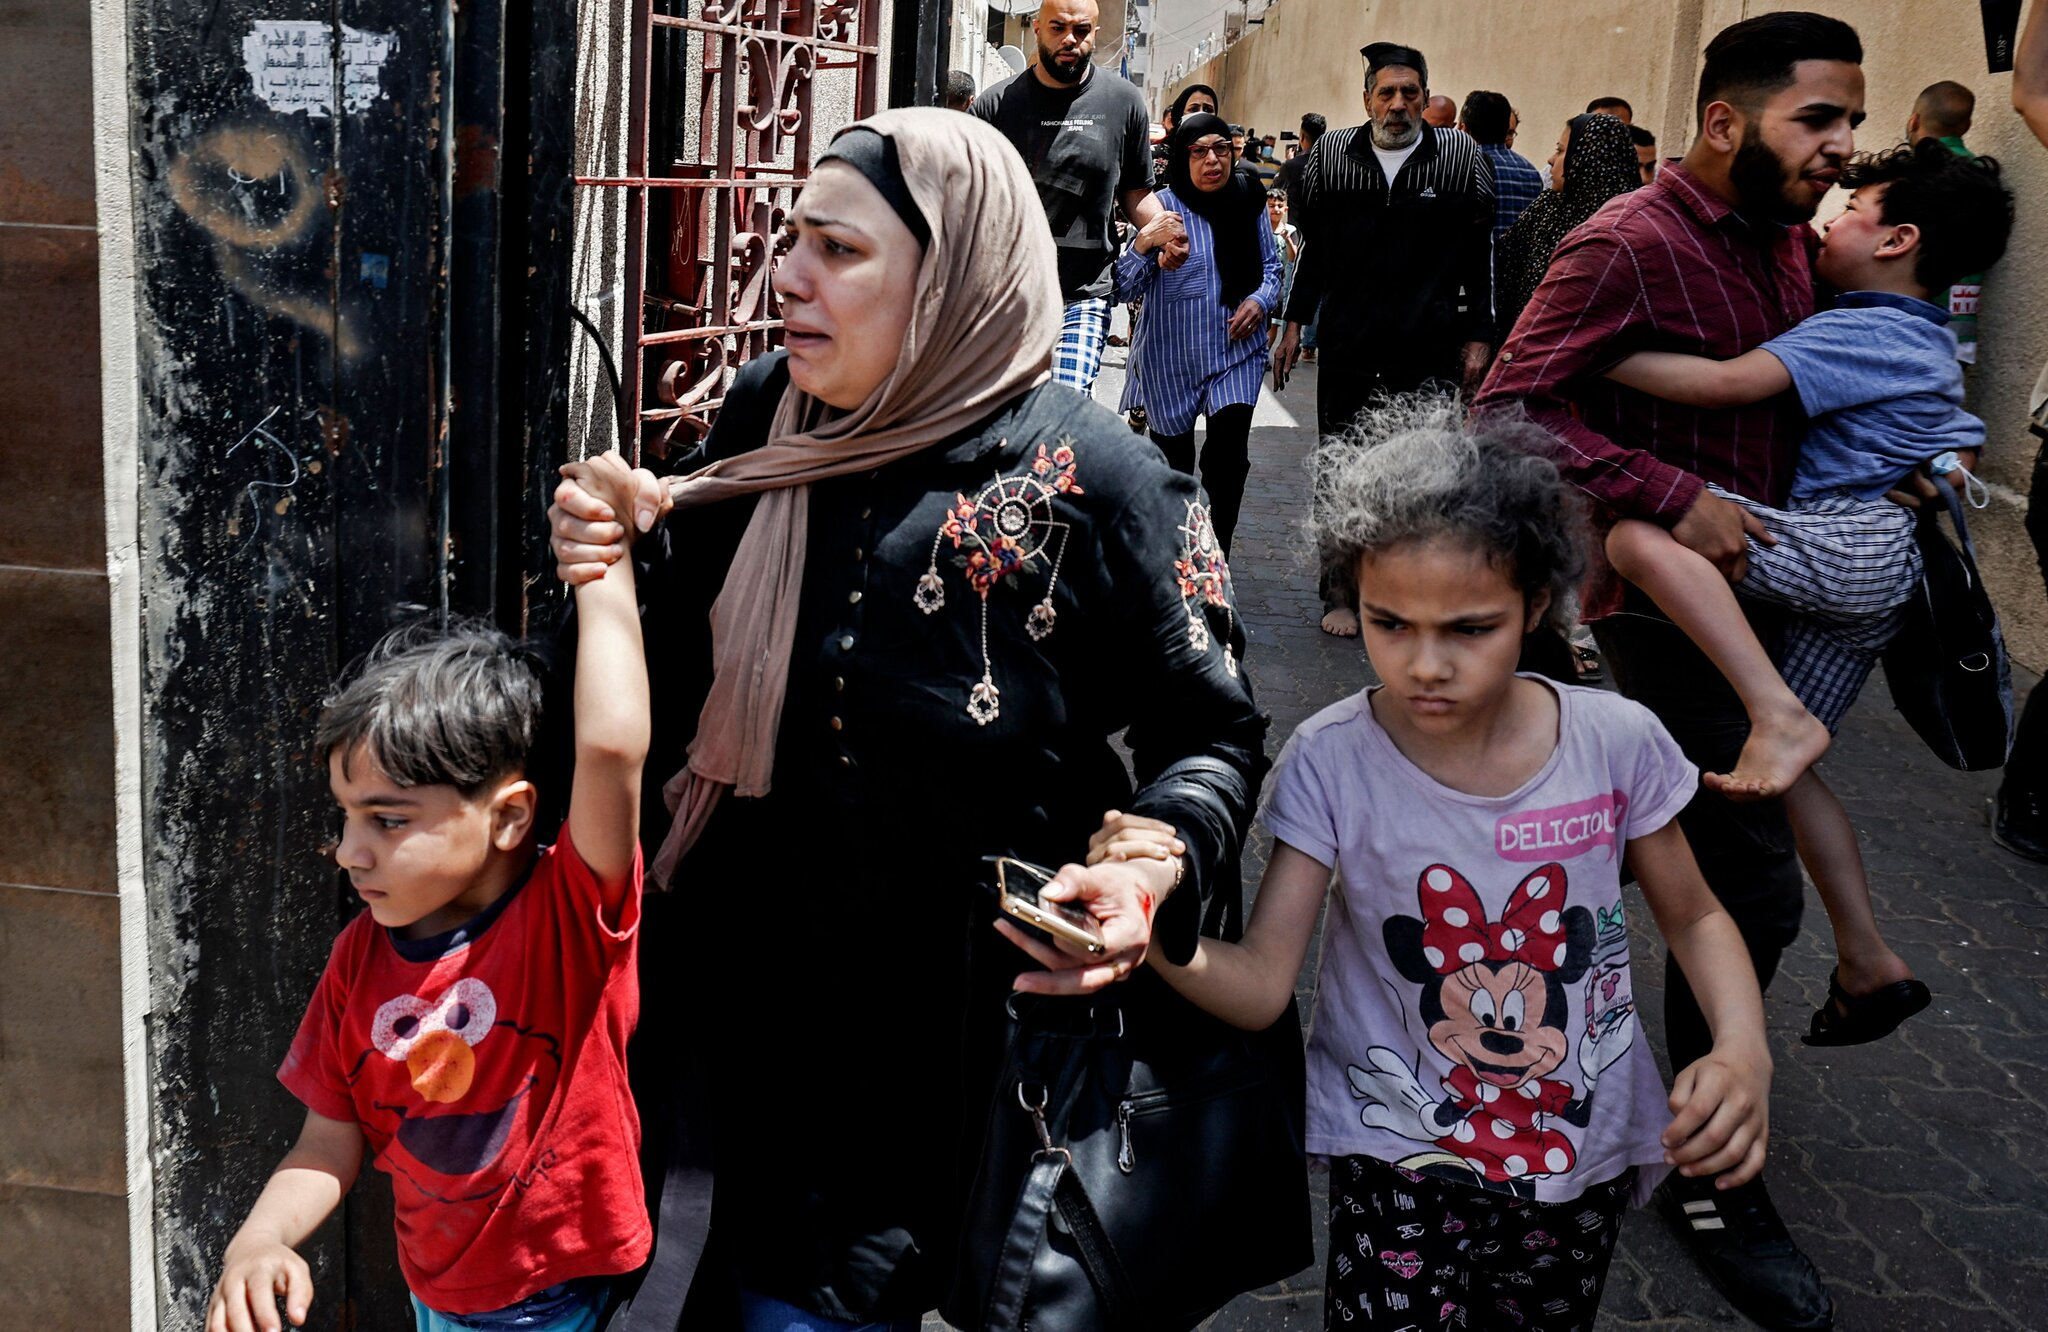
\includegraphics[scale=0.7]{gaza-may-11-2021.jpeg}

Things change slowly in Angelic Worlds too.  When I was youthful, in New York, and had the company of left intellectuals married, we were all familiar with Edward Said's {\em Orientalism} and his other books about issues of newspaper coverage of Islam.  Later, Israel's Mossad blew up Twin Towers in September 11, 2001 and successfully blamed Muslims.  Neconservative war plans for 'post-Soviet regime changes' for many Muslim countries entered us into Crusades.  I was quite upset when in 2008 Israel started doing horrific amounts of 
damage to Palestinians.  Today I have a different perspective.  I think these things are just slow and until there is a recognition of unity of a Single Human Race not much will change quickly.  It is primitive to me for Human Race to believe in racial differences in the first place.  I have shown ethnic influences on moral values and preferences are negligible.  I have shown every ethnicity has almost identical spectrum of good and bad people.  That is the key point; some of these conflicts are hiding great primitive backwardness in Human Race and will continue till these deeper truths of Single Human Race are absorbed.


\end{document}